\documentclass[a4paper]{article}

\usepackage[utf8]{inputenc}

\usepackage{url}
\usepackage[]{hyperref}

\usepackage{caption}

\usepackage{listings}

\usepackage{color}

\usepackage{pythonhighlight}

% *** GRAPHICS RELATED PACKAGES ***
%\usepackage[pdftex]{graphicx}
\usepackage{graphicx}
%\usepackage[dvips]{graphicx}
% to place figures on a fixed position
\usepackage{float}

\usepackage[margin=1in]{geometry}

\title{Hyperbolic Geometry of Complex Networks – Queuing Theory I. Home Assignment II.}
\author{Ferenc Nandor Janky - OA8AT9}
\date{}


\begin{document}

\maketitle

\tableofcontents

\section{Introduction}

The task was to study section I, II, III and IV A of~\cite{HyperbolicGeoNetworks} and in any programming language/tool generate a network according to the model described in the paper 
(in Section IV.A.) with the following parameters: N=5000 (the number of nodes), R=14 (the radius of the disk on which the nodes are uniformly distributed). Then calculate numerically the empirical average degree, and plot on a log-log scale the empirical degree distribution of this generated network.

\section{Implementation}
The implementation of the graph generation and analysis has been done in Python language. The software is available on \url{https://github.com/fecjanky/QT_home_assignment/blob/master/ha2/toki2.py}.
The graph generation has been implemented as described in ~\cite{HyperbolicGeoNetworks}. The node density on the disc with radius \emph{R} along the radial polar coordinates followed an exponential distribution $ \rho~(r) \simeq e^r $~.
The connection probability functions was based on the hyperbolic distance between nodes on the disc given by: $ p(x) = \Theta(R - x) $
For the implementation the following Python libraries have been utilized:
\begin{itemize}
\item \verb!matplotlib! , for creating the representation of the generated graph in polar coordinates and for plotting the degree distribution
\item \verb!networkx! , for graph analysis
\end{itemize}

The  generator function of the points is show in listing~\ref{lst:python}. There were some offset between the simulated and theoretical results (see Section~\ref{sect:metrics}) and it could have been caused by a bias in the generation of random nodes.

\newpage

\begin{lstlisting}[style=mypython,caption={The function used for generating random nodes},label={lst:python}]
    def lte(a, b):
        return math.isclose(a, b) or a < b
	
    # use rejection sampling to generate points with a given distribution
    def generate_points(self, distribution=None):
        points = []
        if distribution is None:
            distribution = lambda r: math.sinh(r) / (math.cosh(self.radius) - 1)

        for i in range(0, self.nodecount):
            azimuth = random.uniform(0, 2 * math.pi)
            d_point = (random.uniform(0, self.radius), random.uniform(0, distribution(self.radius)))
            while True:
                d_accept = distribution(d_point[0])
                if lte(d_point[1], d_accept):
                    break
                d_point = (random.uniform(0, self.radius), random.uniform(0, distribution(self.radius)))
            points.append(PolarPoint(radius=d_point[0], azimuth=azimuth))
        return points
\end{lstlisting}

\section{Results}
\subsection{Theoretical metrics}
To calculate the theoretical average degree the following equations were used from \cite{HyperbolicGeoNetworks}:

\begin{equation}
N = \nu~e^{R/2} \rightarrow \nu \simeq 4.559 ,if\;R=14\;and\;N=5000
\end{equation}
\begin{equation}
R = 2 \ln[8 N / (\pi \overline{k})] \rightarrow \overline{k} \simeq 11.61, if\;R=14\;and\;N=5000
\end{equation}

\subsection{Empirical metrics}\label{sect:metrics}

The polar plot of the generated network can be seen on Figure~\ref{fig:graph}. The empirical average degree calculated for the generated graph was:
\begin{equation}
\overline{k} =  11.8084
\end{equation}

The relative error between the average obtained from the generated one and the theoretical average was:
\begin{equation}
\epsilon = \frac{\vert \overline{k} - \overline{k}_{sim} \vert}{\overline{k} } * 100 \% = 1.71 \%
\end{equation}

\begin{figure}[H]
    \centering
    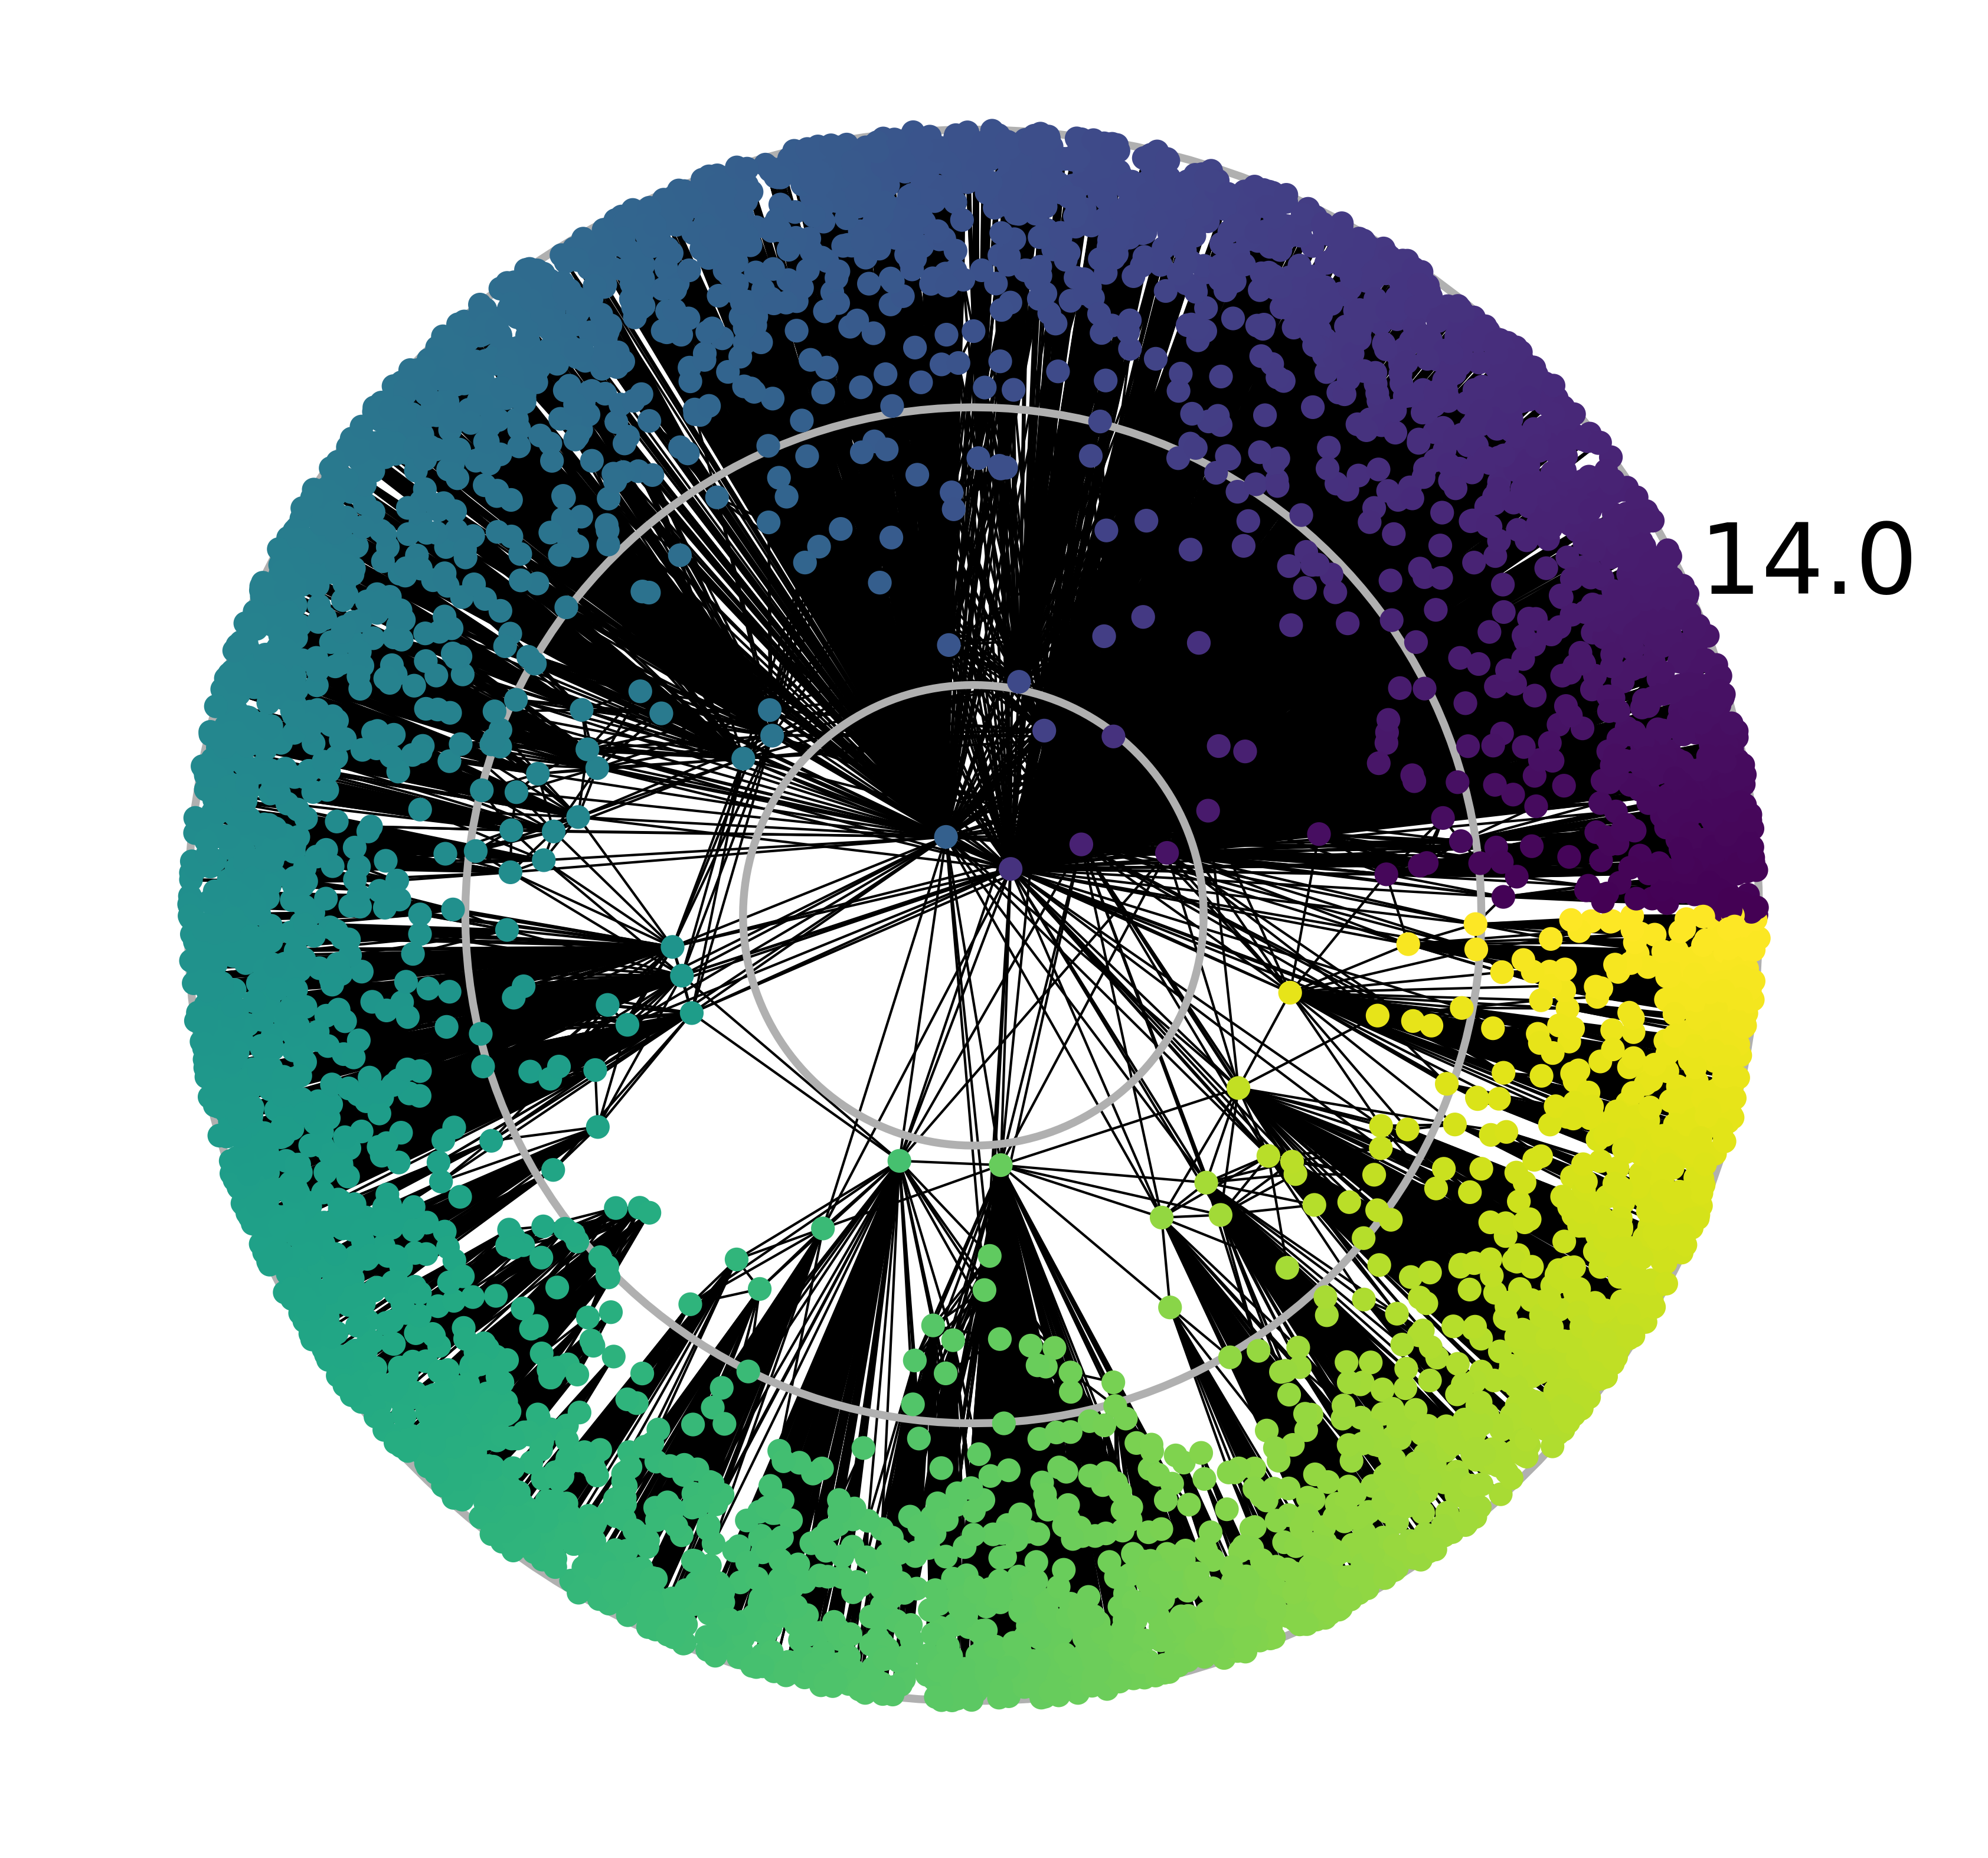
\includegraphics[width=0.9\textwidth]{figures/result_graph.png}
    \caption{The polar plot of the generated graph according to the rules in \cite{HyperbolicGeoNetworks}}
    \label{fig:graph}
\end{figure}


Figure~\ref{fig:graph_stats} shows the empirical degree distribution of the generated network on a log-log scale. It resembles the expected Poissonian distribution.
 
\begin{figure}[H]
    \centering
    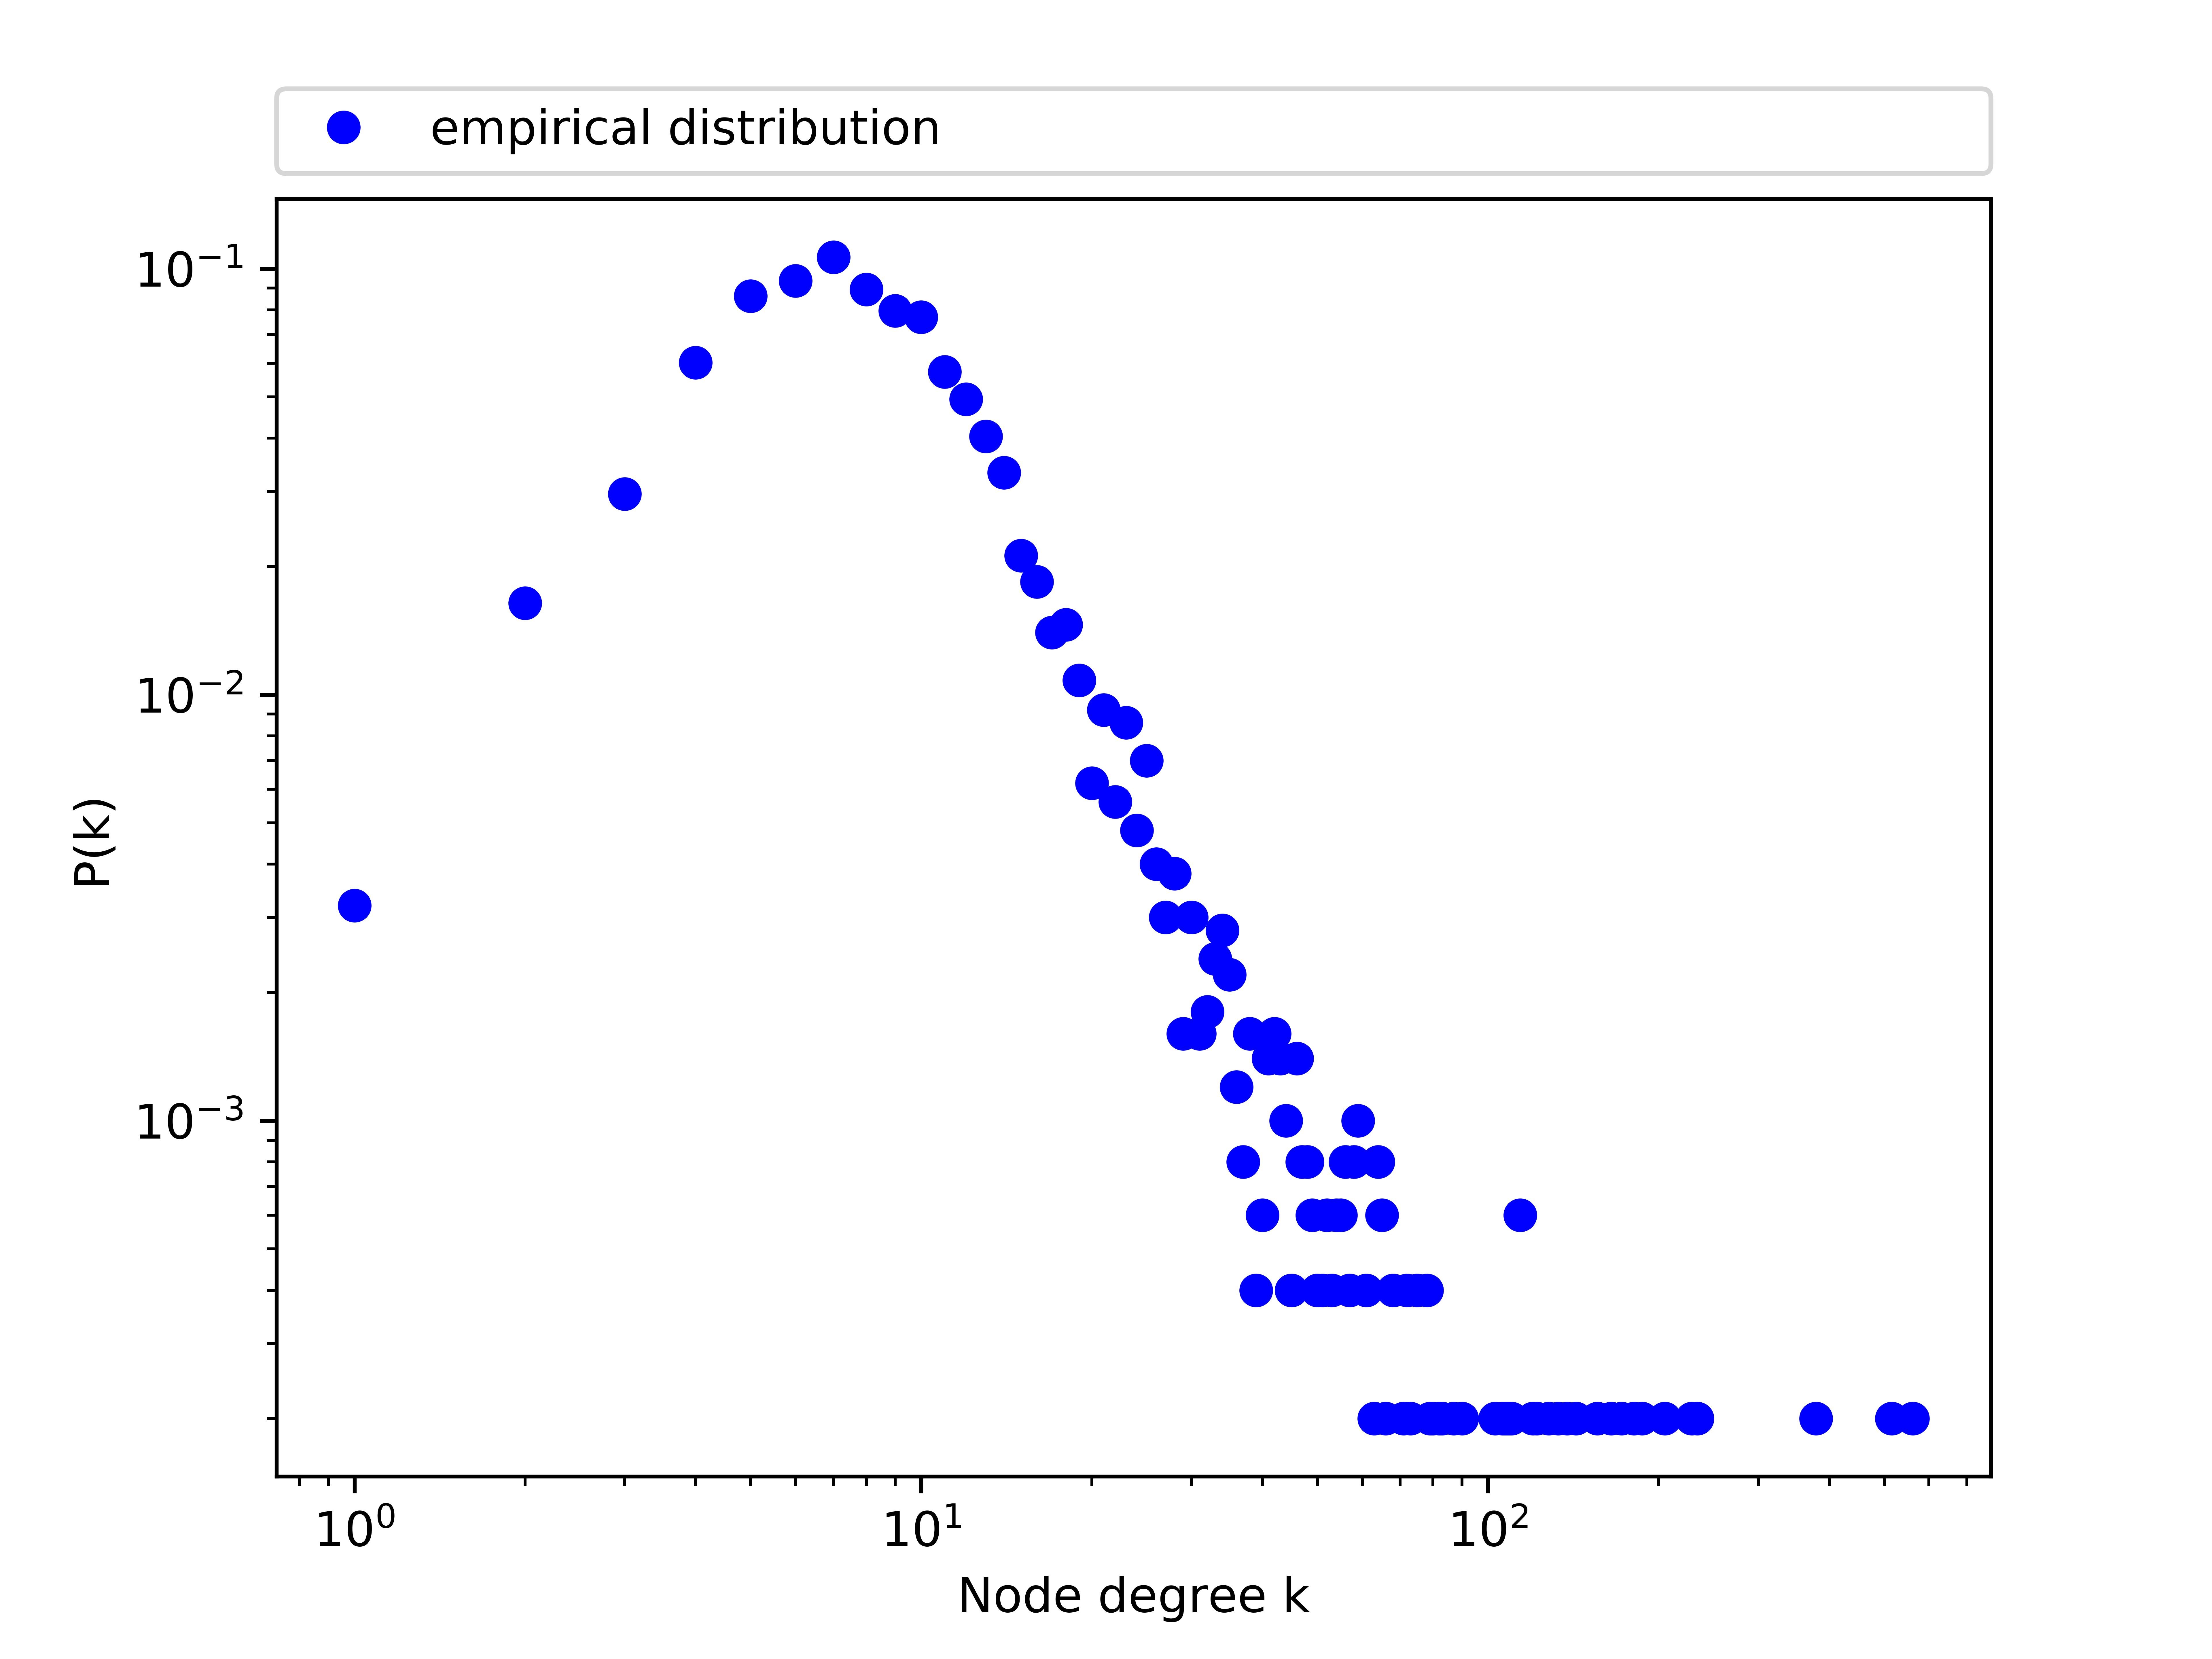
\includegraphics[width=0.9\textwidth]{figures/result_graph_stats.png}
    \caption{The plot on a log-log scale of the empirical degree distribution of the generated network}
    \label{fig:graph_stats}
\end{figure}


The average degree as a function of radius from the center on the disc is illustrated on Figure~\ref{fig:graph_radius} alongside with the theoretical curve. The tangent of the empirical curve is similar however there was a constant offset between them that might have been cause by the bias in the random point generation.

\begin{figure}[H]
    \centering
    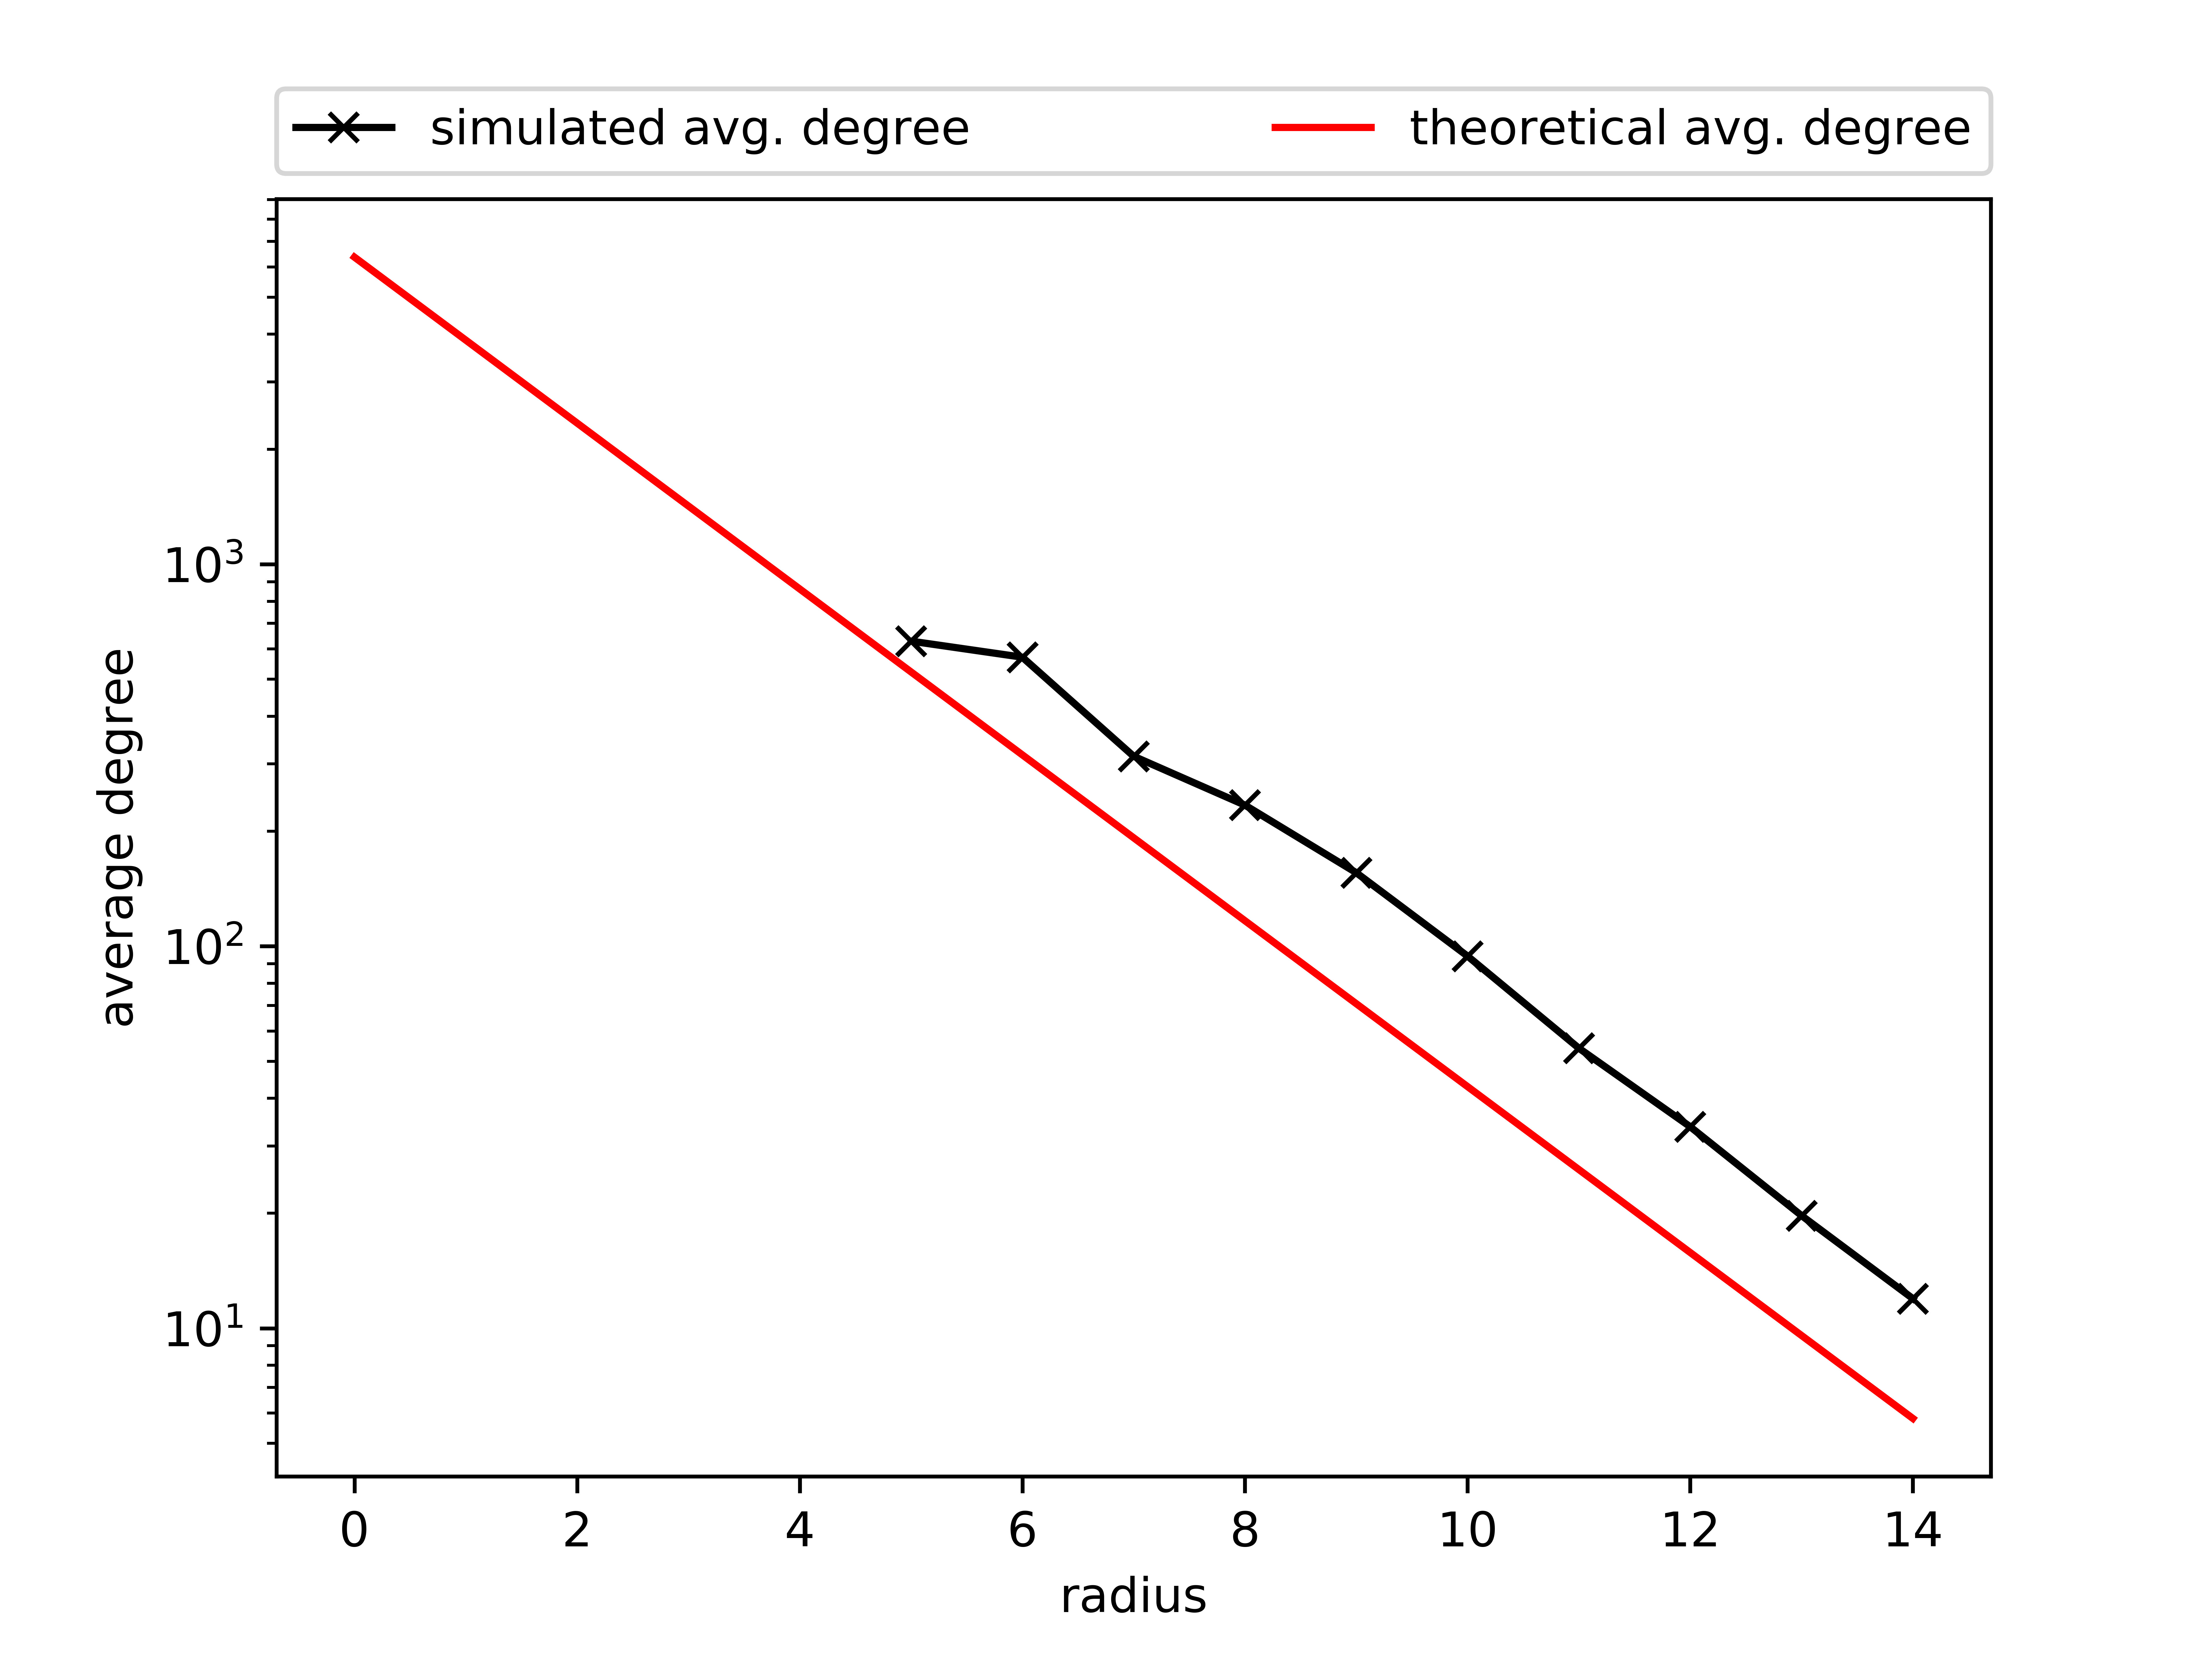
\includegraphics[width=0.9\textwidth]{figures/result_graph_radial_stats.png}
    \caption{The plot of the average degree as a function of radial distance of the generated network}
    \label{fig:graph_radius}
\end{figure}




\section{Conclusion}

As a part of this homework a random network has been generated using  hyperbolic geometry based on \cite{HyperbolicGeoNetworks} to study the
structure and function of complex network in purely geometric terms. The edge probability is analogous to the hyperbolic distance between two nodes and if that distance is below a threshold between 
any of two nodes and edge is present between them.
The simulation results were resembling the theoretical results and also the ones presented in \cite{HyperbolicGeoNetworks} with around 2\% relative error.


\bibliographystyle{unsrt}
\bibliography{references}

\end{document}